\subsection{Premi::Back-End}
	\subsubsection{Informazioni sul package}
		\begin{figure}[h]
			\centering
			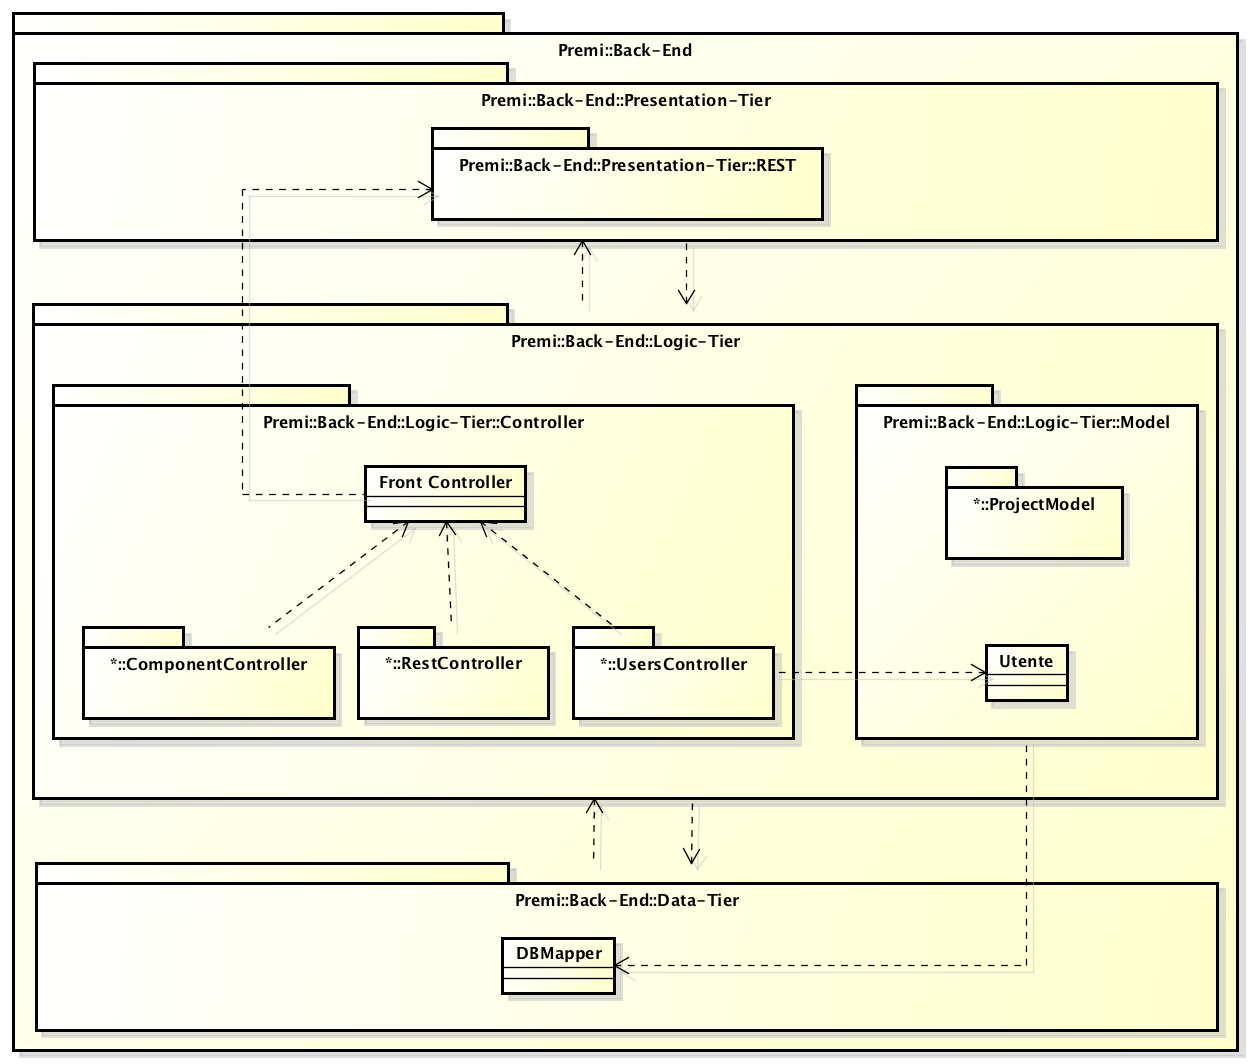
\includegraphics[width=\linewidth]{img/back-end-package}
			\caption[Premi::Back-End]{Premi::Back-End}
		\end{figure}
		Il package contiene le componenti della parte di back-end dell'applicazione.
		
	\subsubsection{Package contenuti}
		\begin{itemize}
			\item *::Presentation-Tier
			\item *::Logic-Tier
			\item *::Data-Tier
		\end{itemize}


\subsection{Premi::Back-End::Presentation-Tier}
	\subsubsection{Informazioni sul package}
		\begin{figure}[h]
			\centering
			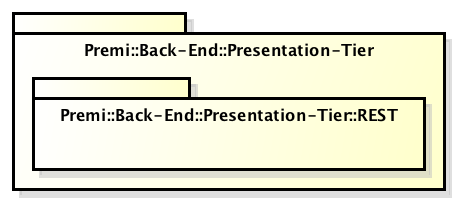
\includegraphics[width=0.7\linewidth]{img/back-end-package_presentation-tier}
			\caption[Premi::Back-End::Presentation-Tier]{Premi::Back-End::Presentation-Tier}
		\end{figure}
		Il package contiene le componenti necessarie per consentire il funzionamento del servizio REST, in modo tale da rendere possibile l'interfacciamento con il front-end.
		
	\subsubsection{Package contenuti}
		\begin{itemize}
			\item *::REST
			\begin{itemize}
				\item Descrizione: Il package contiene la struttura necessaria al funzionamento dell'architettura REST.
			\end{itemize}
		\end{itemize}
		
		
\subsection{Premi::Back-End::Logic-Tier}
	\subsubsection{Informazioni sul package}
	\begin{figure}[h]
		\centering
		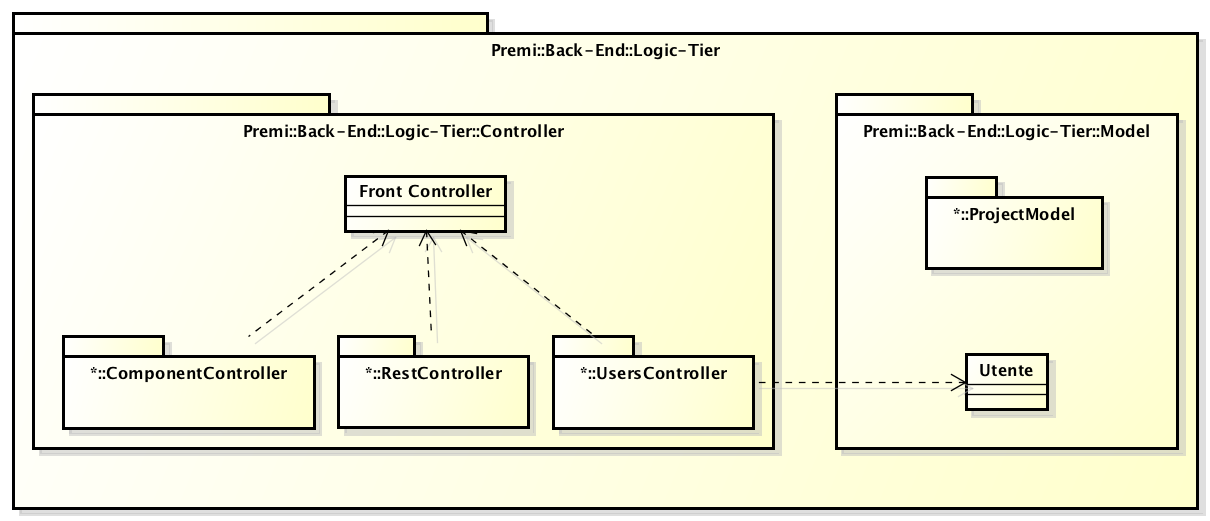
\includegraphics[width=0.7\linewidth]{img/back-end-package_logic-tier}
		\caption[Premi::Back-End::Logic-Tier]{Premi::Back-End::Logic-Tier}
	\end{figure}
	Il package contiene le componenti che si occupano di ricevere le richieste dal Presentation-Tier e di elaborarle attraverso il controller.
	
	\subsubsection{Package contenuti}
	\begin{itemize}
		\item *::Controller
		\item *::Model
	\end{itemize}
	
\newpage
\subsection{Premi::Back-End::Logic-Tier::Model}
	\subsubsection{Informazioni sul package}
	\begin{figure}[h]
	\centering
	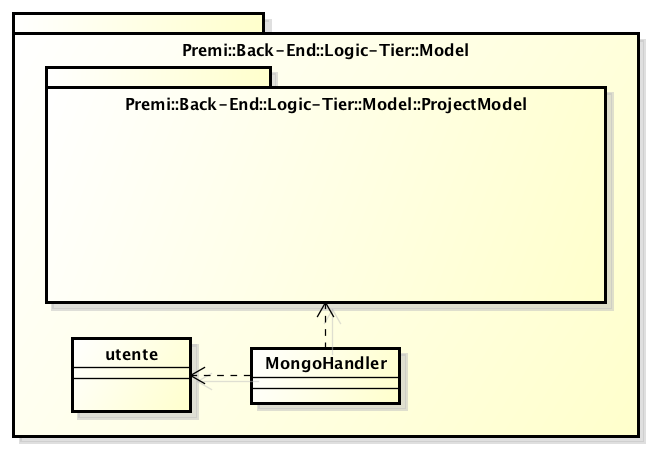
\includegraphics[width=0.9\linewidth]{img/back-end-logic-tier-model}
	\caption[Premi::Back-End::Logic-Tier::Model]{Premi::Back-End::Logic-Tier::Model}
	\end{figure}
	Il package contiene le classi che definisco il modello dell'applicazione.
	
	\subsubsection{Classi contenute}
	\begin{itemize}
		\item \textit{MongoHandler: }serve per comunicare con il livello inferiore ed interagire direttamente con la base di dati;
			\\Relazione con altre classi:
			\begin{itemize}
				\item Premi::Back-End::Logic-Tier::Controller::UsersController::UserController.
			\end{itemize}
		\item \textit{Utente: }fornisce le operazioni per gestire un utente.
			\\Relazione con altre classi:
			\begin{itemize}
				\item Premi::Back-End::Data-Tier::DataTierFrontController.
			\end{itemize}
	\end{itemize}
	
	\subsubsection{Package Contenuti}
	\begin{itemize}
		\item *::ProjectModel.
	\end{itemize}

\newpage	
\subsection{Premi::Back-End::Logic-Tier::Model::ProjectModel}
	\subsubsection{Informazioni sul package}
		\begin{figure}[h]
		\centering
		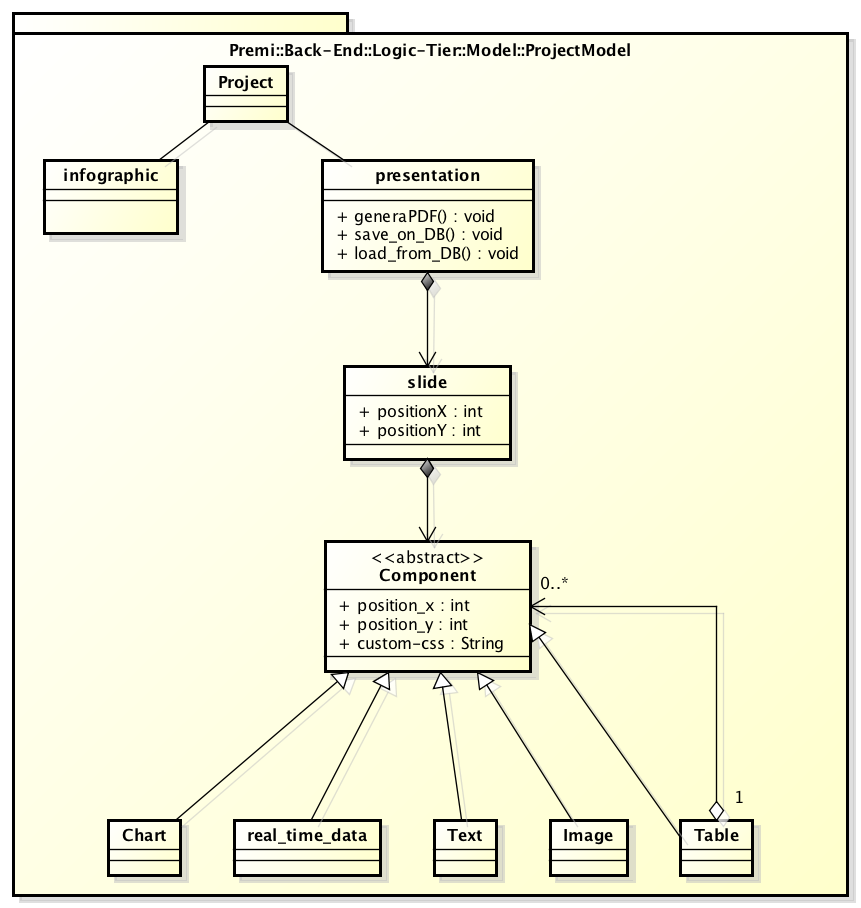
\includegraphics[width=0.9\linewidth]{img/back-end-logic-tier-model-projectModel}
		\caption[Premi::Back-End::Logic-Tier::Model::ProjectModel]{Premi::Back-End::Logic-Tier::Model::ProjectModel}
		\end{figure}
	Il package contiene il modello di tutte le componenti necessarie per il corretto funzionamento dell'applicazione.



